\documentclass[11pt,a4paper]{report}
\usepackage[textwidth=37em,vmargin=30mm]{geometry}
\usepackage{calc,xunicode,amsmath,amssymb,paralist,enumitem,tabu,booktabs,datetime2,xeCJK,xeCJKfntef,listings}
\usepackage{tocloft,fancyhdr,tcolorbox,xcolor,graphicx,eso-pic,xltxtra,xelatexemoji}

\newcommand{\envyear}[0]{2025}
\newcommand{\envdatestr}[0]{2025-05-23}
\newcommand{\envfinaldir}[0]{webdb/2025/20250523/final}

\usepackage[hidelinks]{hyperref}
\hypersetup{
    colorlinks=false,
    pdfpagemode=FullScreen,
    pdftitle={Web Digest - \envdatestr}
}

\setlength{\cftbeforechapskip}{10pt}
\renewcommand{\cftchapfont}{\rmfamily\bfseries\large\raggedright}
\setlength{\cftbeforesecskip}{2pt}
\renewcommand{\cftsecfont}{\sffamily\small\raggedright}

\setdefaultleftmargin{2em}{2em}{1em}{1em}{1em}{1em}

\usepackage{xeCJK,xeCJKfntef}
\xeCJKsetup{PunctStyle=plain,RubberPunctSkip=false,CJKglue=\strut\hskip 0pt plus 0.1em minus 0.05em,CJKecglue=\strut\hskip 0.22em plus 0.2em}
\XeTeXlinebreaklocale "zh"
\XeTeXlinebreakskip = 0pt


\setmainfont{Brygada 1918}
\setromanfont{Brygada 1918}
\setsansfont{IBM Plex Sans}
\setmonofont{JetBrains Mono NL}
\setCJKmainfont{Noto Serif CJK SC}
\setCJKromanfont{Noto Serif CJK SC}
\setCJKsansfont{Noto Sans CJK SC}
\setCJKmonofont{Noto Sans CJK SC}

\setlength{\parindent}{0pt}
\setlength{\parskip}{8pt}
\linespread{1.15}

\lstset{
	basicstyle=\ttfamily\footnotesize,
	numbersep=5pt,
	backgroundcolor=\color{black!5},
	showspaces=false,
	showstringspaces=false,
	showtabs=false,
	tabsize=2,
	captionpos=b,
	breaklines=true,
	breakatwhitespace=true,
	breakautoindent=true,
	linewidth=\textwidth
}






\newcommand{\coverpic}[2]{
    % argv: itemurl, authorname
    Cover photo by #2~~(\href{#1}{#1})
}
\newcommand{\makeheader}[0]{
    \begin{titlepage}
        % \newgeometry{hmargin=15mm,tmargin=21mm,bmargin=12mm}
        \begin{center}
            
            \rmfamily\scshape
            \fontspec{BaskervilleF}
            \fontspec{Old Standard}
            \fontsize{59pt}{70pt}\selectfont
            WEB\hfill DIGEST
            
            \vfill
            % \vskip 30pt
            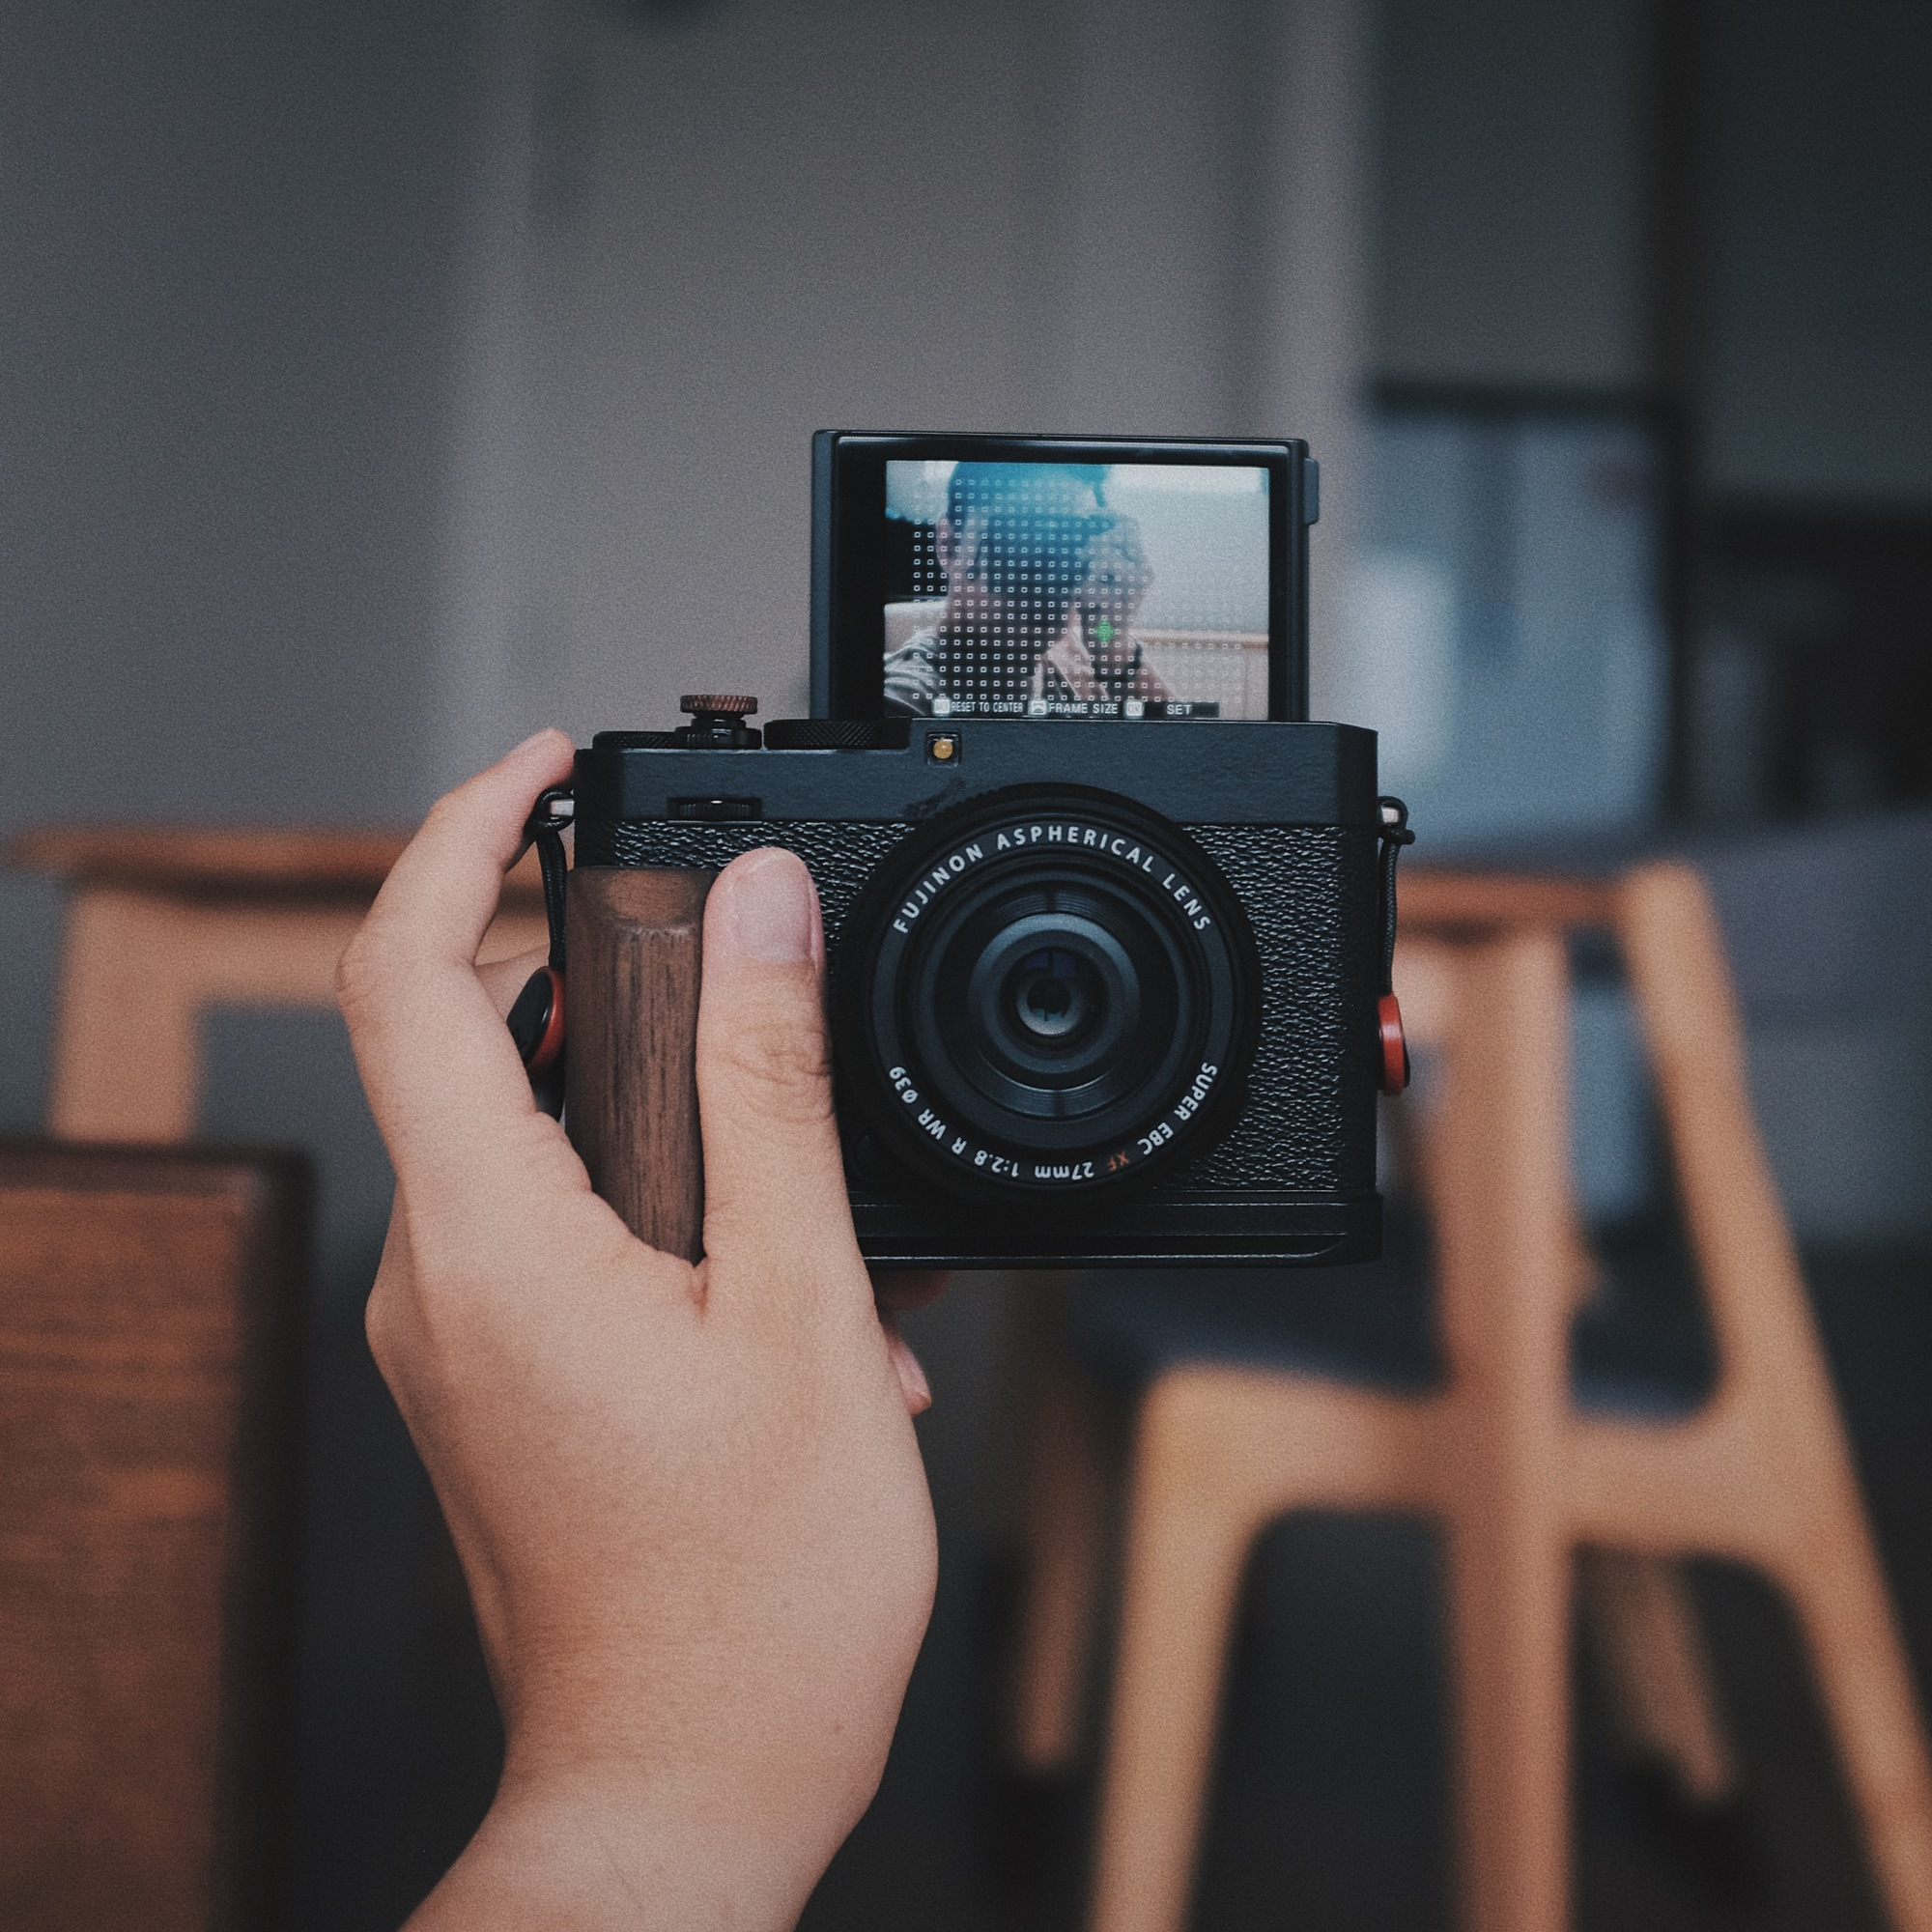
\includegraphics[width=\linewidth]{\envfinaldir/coverpic-prod.jpg}\par
            % \vskip 30pt
            \vfill

            \normalsize\rmfamily\scshape
            \copyright{} The Web Digest Project \hfill\large \envdatestr
        \end{center}
    \end{titlepage}
    % \restoregeometry
}
\newcommand{\simplehref}[1]{%
    \textcolor{blue!80!green}{\href{#1}{#1}}%
}
\renewcommand{\contentsname}{\center\Huge\sffamily\bfseries Contents\par\vskip 20pt}
\newcounter{ipartcounter}
\setcounter{ipartcounter}{0}
\newcommand{\ipart}[1]{
    % \vskip 20pt
    \clearpage
    \stepcounter{ipartcounter}
    \phantomsection
    \addcontentsline{toc}{chapter}{#1}
    % \begin{center}
    %     \Huge
    %     \sffamily\bfseries
    %     #1
    % \end{center}
    % \vskip 20pt plus 7pt
}
\newcounter{ichaptercounter}
\setcounter{ichaptercounter}{0}
\newcommand{\ichapter}[1]{
    % \vskip 20pt
    \clearpage
    \stepcounter{ichaptercounter}
    \phantomsection
    \addcontentsline{toc}{section}{\numberline{\arabic{ichaptercounter}}#1}
    \begin{center}
        \Huge
        \sffamily\bfseries
        #1
    \end{center}
    \vskip 20pt plus 7pt
}
\newcommand{\entrytitlefont}[1]{\subsection*{\raggedright\Large\sffamily\bfseries#1}}
\newcommand{\entryitemGeneric}[2]{
    % argv: title, url
    \parbox{\linewidth}{
        \entrytitlefont{#1}\par\vskip 5pt
        \footnotesize\ttfamily\mdseries
        \simplehref{#2}
    }\vskip 11pt plus 11pt minus 1pt
}
\newcommand{\entryitemGithub}[3]{
    % argv: title, url, desc
    \parbox{\linewidth}{
        \entrytitlefont{#1}\par\vskip 5pt
        \footnotesize\ttfamily\mdseries
        \simplehref{#2}\par\vskip 5pt
        \small\rmfamily\mdseries#3
    }\vskip 11pt plus 11pt minus 1pt
}
\newcommand{\entryitemAp}[3]{
    % argv: title, url, desc
    \parbox{\linewidth}{
        \entrytitlefont{#1}\par\vskip 5pt
        \footnotesize\ttfamily\mdseries
        \simplehref{#2}\par\vskip 5pt
        \small\rmfamily\mdseries#3
    }\vskip 11pt plus 11pt minus 1pt
}
\newcommand{\entryitemHackernews}[3]{
    % argv: title, hnurl, rawurl
    % \parbox{\linewidth}{
    %     \entrytitlefont{#1}\par\vskip 5pt
    %     \footnotesize\ttfamily\mdseries
    %     \simplehref{#3}\par
    %     \textcolor{black!50}{\href{#2}{#2}}
    % }\vskip 11pt plus 11pt minus 1pt
    \begin{minipage}{\linewidth}
            \entrytitlefont{#1}\par\vskip 5pt
            \footnotesize\ttfamily\mdseries
            \simplehref{#3}\par
            \textcolor{black!50}{\href{#2}{#2}}
    \end{minipage}\par\vskip 11pt plus 11pt minus 1pt
}







\begin{document}

\makeheader

\tableofcontents\clearpage




\ipart{Developers}
\ichapter{Hacker News}
\entryitemTwoLinks{Does Earth have two high-tide bulges on opposite sides? (2014)}{https://news.ycombinator.com/item?id=44065458}{http://physics.stackexchange.com/questions/121830/does-earth-really-have-two-high-tide-bulges-on-opposite-sides}

\entryitemTwoLinks{Trump administration halts Harvard's ability to enroll international students}{https://news.ycombinator.com/item?id=44064631}{https://www.nytimes.com/2025/05/22/us/politics/trump-harvard-international-students.html}

\entryitemTwoLinks{Claude 4}{https://news.ycombinator.com/item?id=44063703}{https://www.anthropic.com/news/claude-4}

\entryitemTwoLinks{Mozilla to shut down Pocket on July 8}{https://news.ycombinator.com/item?id=44063662}{https://support.mozilla.org/en-US/kb/future-of-pocket}

\entryitemTwoLinks{That fractal that's been up on my wall for 12 years}{https://news.ycombinator.com/item?id=44063248}{https://chriskw.xyz/2025/05/21/Fractal/}

\entryitemTwoLinks{MCP explained without hype or fluff}{https://news.ycombinator.com/item?id=44063141}{https://blog.nilenso.com/blog/2025/05/12/mcp-explained-without-hype-or-fluff/}

\entryitemTwoLinks{U.S. Spy Agencies–One-Stop Shop to Buy Your Personal Data}{https://news.ycombinator.com/item?id=44062586}{https://theintercept.com/2025/05/22/intel-agencies-buying-data-portal-privacy/}

\entryitemTwoLinks{I Built My Own Audio Player}{https://news.ycombinator.com/item?id=44062227}{https://nexo.sh/posts/why-i-built-a-native-mp3-player-in-swiftui/}

\entryitemTwoLinks{Fast Allocations in Ruby 3.5}{https://news.ycombinator.com/item?id=44062160}{https://railsatscale.com/2025-05-21-fast-allocations-in-ruby-3-5/}

\entryitemTwoLinks{Show HN: SQLite JavaScript - extend your database with JavaScript}{https://news.ycombinator.com/item?id=44061836}{https://github.com/sqliteai/sqlite-js}

\entryitemTwoLinks{Improving performance of rav1d video decoder}{https://news.ycombinator.com/item?id=44061160}{https://ohadravid.github.io/posts/2025-05-rav1d-faster/}

\entryitemTwoLinks{Planetfall}{https://news.ycombinator.com/item?id=44060305}{https://somethingaboutmaps.wordpress.com/2025/05/20/planetfall/}

\entryitemTwoLinks{Why does Debian change software?}{https://news.ycombinator.com/item?id=44059411}{https://blog.liw.fi/posts/2025/why-debian-changes/}

\entryitemTwoLinks{The scientific ``unit'' we call the decibel}{https://news.ycombinator.com/item?id=44058778}{https://lcamtuf.substack.com/p/decibels-are-ridiculous}

\entryitemTwoLinks{ChatGPT Is a Gimmick}{https://news.ycombinator.com/item?id=44058677}{https://hedgehogreview.com/web-features/thr/posts/chatgpt-is-a-gimmick}

\entryitemTwoLinks{Kotlin-Lsp: Kotlin Language Server and Plugin for Visual Studio Code}{https://news.ycombinator.com/item?id=44058299}{https://github.com/Kotlin/kotlin-lsp}

\entryitemTwoLinks{Getting a paper accepted}{https://news.ycombinator.com/item?id=44057841}{https://maxwellforbes.com/posts/how-to-get-a-paper-accepted/}

\entryitemTwoLinks{Gemini Diffusion}{https://news.ycombinator.com/item?id=44057820}{https://simonwillison.net/2025/May/21/gemini-diffusion/}

\entryitemTwoLinks{Display any CSV file as a searchable, filterable, pretty HTML table}{https://news.ycombinator.com/item?id=44057612}{https://github.com/derekeder/csv-to-html-table}

\entryitemTwoLinks{Should I Block ICMP?}{https://news.ycombinator.com/item?id=44057219}{http://shouldiblockicmp.com/}\ichapter{Phoronix}
\entryitemGeneric{\hskip 0pt{}SteamOS 3.7 Stable Rolls Out With Updated Linux Kernel, Expanding AMD Handheld Support}{https://www.phoronix.com/news/SteamOS-3.7.8-Stable}

\entryitemGeneric{\hskip 0pt{}Ubuntu 25.10 Switching To Chrony By Default, Enabling Network Time Security}{https://www.phoronix.com/news/Ubuntu-25.10-Chrony}

\entryitemGeneric{\hskip 0pt{}Mozilla Is Shutting Down Pocket}{https://www.phoronix.com/news/Mozilla-Pocket-Ending}

\entryitemGeneric{\hskip 0pt{}Canonical Planning For Linux 6.17 To Power Ubuntu 25.10}{https://www.phoronix.com/news/Ubuntu-25.10-With-Linux-6.17}

\entryitemGeneric{\hskip 0pt{}Intel Announces New Xeon 6 CPU Models With SST-TF \& Priority Core Turbo "PCT"}{https://www.phoronix.com/news/Intel-Xeon-6-SST-TF-PCT}

\entryitemGeneric{\hskip 0pt{}Maximizing The Performance \& Power Efficiency Of AMD Ryzen AI Max+ 395 With Platform Profiles}{https://www.phoronix.com/review/amd-strix-halo-platform-profile}

\entryitemGeneric{\hskip 0pt{}PoCL 7.0 Released With Official OpenCL 3.0 Conformance On x86\_64 CPUs}{https://www.phoronix.com/news/PoCL-7.0-Released}

\entryitemGeneric{\hskip 0pt{}FFmpeg FFV1 Vulkan Encoder Lands +35\% Improvement For AMD, +50\% For NVIDIA}{https://www.phoronix.com/news/FFmpeg-Faster-FFV1-Vulkan-Enc}

\entryitemGeneric{\hskip 0pt{}AMD Preparing For Some Nice GPU Reset Improvements Under Linux}{https://www.phoronix.com/news/Better-AMD-GPU-Reset-Linux}\ichapter{Dribbble}
\entryitemGeneric{\hskip 0pt{}Smart Home App}{https://dribbble.com/shots/26056748-Smart-Home-App}

\entryitemGeneric{\hskip 0pt{}Illustration}{https://dribbble.com/shots/26052539-Illustration}

\entryitemGeneric{\hskip 0pt{}Travel Startup Branding for Holidu: visual identity brand design}{https://dribbble.com/shots/25983747-Travel-Startup-Branding-for-Holidu-visual-identity-brand-design}

\entryitemGeneric{\hskip 0pt{}Playground web interaction}{https://dribbble.com/shots/26048246-Playground-web-interaction}

\entryitemGeneric{\hskip 0pt{}Onday - Logo Design}{https://dribbble.com/shots/26053436-Onday-Logo-Design}

\entryitemGeneric{\hskip 0pt{}DICH™ Fashion Vol.2}{https://dribbble.com/shots/26046875-DICH-Fashion-Vol-2}

\entryitemGeneric{\hskip 0pt{}L'Renee \& Associates logo}{https://dribbble.com/shots/26047943-L-Renee-Associates-logo}

\entryitemGeneric{\hskip 0pt{}Magus Logo Design}{https://dribbble.com/shots/26048055-Magus-Logo-Design}

\entryitemGeneric{\hskip 0pt{}Chromix – Logo Design // For Sale}{https://dribbble.com/shots/26048061-Chromix-Logo-Design-For-Sale}

\entryitemGeneric{\hskip 0pt{}F}{https://dribbble.com/shots/26041370-F}

\entryitemGeneric{\hskip 0pt{}Mackerel}{https://dribbble.com/shots/26043994-Mackerel}

\entryitemGeneric{\hskip 0pt{}Howdy from a happy hermit!}{https://dribbble.com/shots/26043217-Howdy-from-a-happy-hermit}

\entryitemGeneric{\hskip 0pt{}Dark or Light?}{https://dribbble.com/shots/26042325-Dark-or-Light}

\entryitemGeneric{\hskip 0pt{}Evergreen}{https://dribbble.com/shots/26042187-Evergreen}

\entryitemGeneric{\hskip 0pt{}Planto}{https://dribbble.com/shots/26044620-Planto}

\entryitemGeneric{\hskip 0pt{}Ebay Rebranding Concept}{https://dribbble.com/shots/26039712-Ebay-Rebranding-Concept}

\entryitemGeneric{\hskip 0pt{}QueenClub Logo Design}{https://dribbble.com/shots/26042947-QueenClub-Logo-Design}

\entryitemGeneric{\hskip 0pt{}Finance Landing Page Design}{https://dribbble.com/shots/26037973-Finance-Landing-Page-Design}

\entryitemGeneric{\hskip 0pt{}Taskly - Task Management Dashboard}{https://dribbble.com/shots/26031962-Taskly-Task-Management-Dashboard}

\entryitemGeneric{\hskip 0pt{}Profile Card 👧}{https://dribbble.com/shots/26033069-Profile-Card}

\entryitemGeneric{\hskip 0pt{}DICH™ Fashion}{https://dribbble.com/shots/26032014-DICH-Fashion}

\entryitemGeneric{\hskip 0pt{}Techtots on UI8 illustration set}{https://dribbble.com/shots/25995896-Techtots-on-UI8-illustration-set}

\entryitemGeneric{\hskip 0pt{}Letter E + Link Logo Concept}{https://dribbble.com/shots/26032100-Letter-E-Link-Logo-Concept}

\entryitemGeneric{\hskip 0pt{}Watch Face}{https://dribbble.com/shots/26030361-Watch-Face}


\ipart{Developers~~~~(zh-Hans)}
\ichapter{Solidot}
\entryitemGeneric{\hskip 0pt{}OpenAI 以 65 亿美元收购 Jony Ive 创办的 io 公司}{https://www.solidot.org/story?sid=81361}

\entryitemGeneric{\hskip 0pt{}微软称全世界有 39.4 万台 Windows 电脑感染了 Lumma 恶意程序}{https://www.solidot.org/story?sid=81360}

\entryitemGeneric{\hskip 0pt{}Google 搜索关键词历史抓获 2020 年丹佛致命纵火案凶手}{https://www.solidot.org/story?sid=81359}

\entryitemGeneric{\hskip 0pt{}巴西研究人员抓取 20 亿条 Discord 消息公开发布}{https://www.solidot.org/story?sid=81358}

\entryitemGeneric{\hskip 0pt{}新闻标题过去二十年越来越长越来越负面}{https://www.solidot.org/story?sid=81357}

\entryitemGeneric{\hskip 0pt{}Google 的视频生成模型 Veo 3 能同步音频}{https://www.solidot.org/story?sid=81356}

\entryitemGeneric{\hskip 0pt{}天宫空间站拭子发现未知菌种}{https://www.solidot.org/story?sid=81355}

\entryitemGeneric{\hskip 0pt{}猴痘全球疫情爆发前已在尼日利亚传播了八年}{https://www.solidot.org/story?sid=81354}

\entryitemGeneric{\hskip 0pt{}俄罗斯停止公开人口统计数据细节}{https://www.solidot.org/story?sid=81353}

\entryitemGeneric{\hskip 0pt{}IEEE 刊登的一篇论文被发现包含中文脏话}{https://www.solidot.org/story?sid=81352}

\entryitemGeneric{\hskip 0pt{}法国禁止 Telegram 创始人 Pavel Durov 前往美国}{https://www.solidot.org/story?sid=81350}

\entryitemGeneric{\hskip 0pt{}报纸刊登的推荐书单名被发现多数是 AI 捏造的}{https://www.solidot.org/story?sid=81349}

\entryitemGeneric{\hskip 0pt{}美国大学城走向萧条}{https://www.solidot.org/story?sid=81348}

\entryitemGeneric{\hskip 0pt{}Google 搜索开始向美国用户提供 AI 模式}{https://www.solidot.org/story?sid=81347}

\entryitemGeneric{\hskip 0pt{}微软封了国际刑事法院首席检察官的电邮账号}{https://www.solidot.org/story?sid=81346}

\entryitemGeneric{\hskip 0pt{}调查发现气候科学家是最不受信任的科学家}{https://www.solidot.org/story?sid=81345}

\entryitemGeneric{\hskip 0pt{}Red Hat 宣布 RHEL 10,推出针对 RISC-V 架构的开发者预览版}{https://www.solidot.org/story?sid=81344}

\entryitemGeneric{\hskip 0pt{}4 月中国智能手机出口暴跌 72\%}{https://www.solidot.org/story?sid=81343}

\entryitemGeneric{\hskip 0pt{}丹麦考虑建造核电}{https://www.solidot.org/story?sid=81342}

\entryitemGeneric{\hskip 0pt{}2024 年电动汽车占到汽车总销量逾五分之一}{https://www.solidot.org/story?sid=81341}\ichapter{V2EX}
\entryitemGeneric{\hskip 0pt{}[酷工作] [远程] [外企 contractor] PostgreSQL DBA 工程师}{https://www.v2ex.com/t/1133681}

\entryitemGeneric{\hskip 0pt{}[TypeScript] TypeScript Native 预览版发布了}{https://www.v2ex.com/t/1133680}

\entryitemGeneric{\hskip 0pt{}[程序员] 太谜了, Chrome 的开发控制台 AI 功能被强行禁用, Gemini 则没问题}{https://www.v2ex.com/t/1133679}

\entryitemGeneric{\hskip 0pt{}[问与答] AI 大乱斗的当下,有没有评测工具可以做下权重标记?}{https://www.v2ex.com/t/1133678}

\entryitemGeneric{\hskip 0pt{}[问与答] 有没有懂哥讲讲小米新出的 CPU 里自主率多高?}{https://www.v2ex.com/t/1133677}

\entryitemGeneric{\hskip 0pt{}[生活] 没事干买了几条女生扎头发的头绳}{https://www.v2ex.com/t/1133676}

\entryitemGeneric{\hskip 0pt{}[奇思妙想] 谷歌 play 印度区 土耳其区 埃及区 YouTube premium 内购提示``无法完成你的购买交易,请前往账户设定,确认账单地址与居住国家相同''}{https://www.v2ex.com/t/1133675}

\entryitemGeneric{\hskip 0pt{}[大学] 在准备 HCI 某会议投稿,但是今天在看去年同一个会议接收的论文的时候发现有一篇综述和我在做的完全同一个方向甚至最后提出的想法、技术栈完全一样,不同的是我是实践这个论文是理论,这种情况下还有机会中稿吗?}{https://www.v2ex.com/t/1133674}

\entryitemGeneric{\hskip 0pt{}[OpenAI] claude4 发布,貌似被灰度到了一个活动}{https://www.v2ex.com/t/1133673}

\entryitemGeneric{\hskip 0pt{}[问与答] 大电视搬家有人弄过吗}{https://www.v2ex.com/t/1133672}

\entryitemGeneric{\hskip 0pt{}[分享创造] Need to Estimate Asphalt for Your Driveway or Parking Lot? Here's a Free Tool I Built}{https://www.v2ex.com/t/1133671}

\entryitemGeneric{\hskip 0pt{}[酷工作] AWS 运维知识请教(200 元每小时)}{https://www.v2ex.com/t/1133670}

\entryitemGeneric{\hskip 0pt{}[推广] 有港卡赶紧把本土羊毛带回家}{https://www.v2ex.com/t/1133668}

\entryitemGeneric{\hskip 0pt{}[分享发现] Claude Opus 4 和 Claude Sonnet 4 现已发布}{https://www.v2ex.com/t/1133667}

\entryitemGeneric{\hskip 0pt{}[奇思妙想] RECCV 检测人脸伪造项目尝试与扩展}{https://www.v2ex.com/t/1133665}

\entryitemGeneric{\hskip 0pt{}[职场话题] 澳洲职场请教}{https://www.v2ex.com/t/1133664}

\entryitemGeneric{\hskip 0pt{}[问与答] 活久见的事,闲鱼转账错了,对方是老赖,一到账就直接被支付宝自动还了借呗,咋办?}{https://www.v2ex.com/t/1133663}

\entryitemGeneric{\hskip 0pt{}[全球工单系统] bitwarden 的端到端加密是否足够可信,使用公共的 vaultwarden 实例安全吗?}{https://www.v2ex.com/t/1133662}

\entryitemGeneric{\hskip 0pt{}[分享发现] 强烈批判某同行拿我们的兑换码转卖盈利以及收集顾客信息}{https://www.v2ex.com/t/1133661}

\entryitemGeneric{\hskip 0pt{}[Apple] surge6 要来了,又要重新订阅购买了}{https://www.v2ex.com/t/1133660}

\entryitemGeneric{\hskip 0pt{}[问与答] 今天看到闲鱼 PR 发在网盘美剧里面插广告,有没有老哥看过这种视频,想见识见识}{https://www.v2ex.com/t/1133659}

\entryitemGeneric{\hskip 0pt{}[分享创造] 在线时间戳(Unix TimeStamp)转换器}{https://www.v2ex.com/t/1133658}

\entryitemGeneric{\hskip 0pt{}[程序员] 小米玄戒 O1 用到了旗舰机且性能达到一线 soc 水平}{https://www.v2ex.com/t/1133657}

\entryitemGeneric{\hskip 0pt{}[服务器] 高防 CDN 和高防服务器的区别}{https://www.v2ex.com/t/1133656}

\entryitemGeneric{\hskip 0pt{}[生活] B 站上那些农村生活类的 up 主真的活得那么舒服么}{https://www.v2ex.com/t/1133654}

\entryitemGeneric{\hskip 0pt{}[问与答] Ubuntu 如何转换为 OPENBSD}{https://www.v2ex.com/t/1133652}

\entryitemGeneric{\hskip 0pt{}[问与答] 看到一篇采访 Spring 之父的文章,很推荐 kotlin,问问大家的看法}{https://www.v2ex.com/t/1133650}

\entryitemGeneric{\hskip 0pt{}[分享发现] 站里刷到个玄学贴,我来为大家试试,用 ``高岛易断'' 预测未来一周 BTC 走势}{https://www.v2ex.com/t/1133649}

\entryitemGeneric{\hskip 0pt{}[生活] 和 AI 沟通心理与情绪问题,对话记录丢失后……}{https://www.v2ex.com/t/1133648}

\entryitemGeneric{\hskip 0pt{}[问与答] cloudflare r2 对象存储,移动无法访问}{https://www.v2ex.com/t/1133647}

\entryitemGeneric{\hskip 0pt{}[问与答] 小米这是往华子更接近了一步?}{https://www.v2ex.com/t/1133646}

\entryitemGeneric{\hskip 0pt{}[酷工作] [京东零售] [组内直招] 软件开发工程师}{https://www.v2ex.com/t/1133645}

\entryitemGeneric{\hskip 0pt{}[iCloud] 您的 Apple ID 被用于在 Web 浏览器上登录 iCloud 自从 2020 年没有邮箱提示}{https://www.v2ex.com/t/1133642}

\entryitemGeneric{\hskip 0pt{}[分享创造] 做了一个 Web+本地文件的 Vibe Coding,欢迎测试和建议,因为这是第一个测试版,功能肯定存在大量缺陷,所以无限制的完全免费(附带功能核心系统提示词)}{https://www.v2ex.com/t/1133641}

\entryitemGeneric{\hskip 0pt{}[杭州] 警惕骗子公司 亲身经历 坐标杭州 再者求职三年前端}{https://www.v2ex.com/t/1133639}

\entryitemGeneric{\hskip 0pt{}[酷工作] 帮朋友招个前端 坐标杭州未来科技城}{https://www.v2ex.com/t/1133634}

\entryitemGeneric{\hskip 0pt{}[问与答] 经济下行的几大好处}{https://www.v2ex.com/t/1133633}

\entryitemGeneric{\hskip 0pt{}[随想] IT 之家首页 73 处'小米' ! 纳闷我们每天摄入的是新闻, 是广告, 还是什么?}{https://www.v2ex.com/t/1133632}

\entryitemGeneric{\hskip 0pt{}[问与答] 大家有没有发现黑色的车身,晚上很容易看走眼}{https://www.v2ex.com/t/1133631}

\entryitemGeneric{\hskip 0pt{}[分享发现] 淘宝造假标签坑害好商家! 180 天零差评竟被改成 90\%好评率,官方傲慢无视商家血汗}{https://www.v2ex.com/t/1133630}

\entryitemGeneric{\hskip 0pt{}[开源软件] [开源] 实时工资计算器 - 看着你每秒都在赚钱}{https://www.v2ex.com/t/1133629}

\entryitemGeneric{\hskip 0pt{}[Notion] Notion AI 涨价了?}{https://www.v2ex.com/t/1133628}

\entryitemGeneric{\hskip 0pt{}[宽带症候群] 中国移动自己把互联网交换中心堵死了,还倒打一耙说 中国电信 中国联通 限制中国移动}{https://www.v2ex.com/t/1133627}

\entryitemGeneric{\hskip 0pt{}[问与答] V2EX Polish 插件停更了?}{https://www.v2ex.com/t/1133626}

\entryitemGeneric{\hskip 0pt{}[程序员] cursor pro 免费 3 个月}{https://www.v2ex.com/t/1133624}

\entryitemGeneric{\hskip 0pt{}[问与答] 求大佬们的国外远程工作建议!}{https://www.v2ex.com/t/1133623}

\entryitemGeneric{\hskip 0pt{}[分享创造] 匿名吐槽+ 阅后即焚的小工具}{https://www.v2ex.com/t/1133621}

\entryitemGeneric{\hskip 0pt{}[远程工作] [招聘] 成熟 Web3 创业团队招资深工程师(远程)}{https://www.v2ex.com/t/1133618}

\entryitemGeneric{\hskip 0pt{}[Windows] win11 LTSC 24H2 是不是和 VMware 不兼容呀}{https://www.v2ex.com/t/1133617}

\entryitemGeneric{\hskip 0pt{}[职场话题] 深圳社保补缴后,以往年份的个人所得税退税流程}{https://www.v2ex.com/t/1133616}


\ipart{Generic News}







\clearpage
\leavevmode\vfill
\footnotesize

Copyright \copyright{} 2023-2025 Neruthes and other contributors.

This document is published with CC BY-NC-ND 4.0 license.

The entries listed in this newsletter may be copyrighted by their respective creators.

This newsletter is generated by the Web Digest project.

The newsletters are also delivered via Telegram channel \CJKunderline{\href{https://t.me/webdigestchannel}{https://t.me/webdigestchannel}}.\\
RSS feed is available at \CJKunderline{\href{https://webdigest.pages.dev/rss.xml}{https://webdigest.pages.dev/rss.xml}}.

This newsletter is available in PDF at
\CJKunderline{\href{https://webdigest.pages.dev/}{https://webdigest.pages.dev/}}.

The source code being used to generate this newsletter is available at\\
\CJKunderline{\href{https://github.com/neruthes/webdigest}{https://github.com/neruthes/webdigest}}.

This newsletter is also available in
\CJKunderline{\href{http://webdigest.pages.dev/readhtml/\envyear/WebDigest-20250523.html}{HTML}} and
\CJKunderline{\href{https://github.com/neruthes/webdigest/blob/master/markdown/\envyear/WebDigest-20250523.md}{Markdown}}.


\coverpic{https://unsplash.com/photos/a-white-van-is-parked-in-front-of-an-auto-shop-sw241wMxJHY}{Danny Greenberg}


\end{document}
